\clearpage
\section{Ultrasonic sensor}

For the autonomous navigation, the rover will be using 3 ultrasonic sensors for close-proximity detection. These sensors will be mounted on the front arc of the rover, at the same height as the wheels to help detect objects within a close distance of the rover.

\begin{figure}[H]
	\centering
	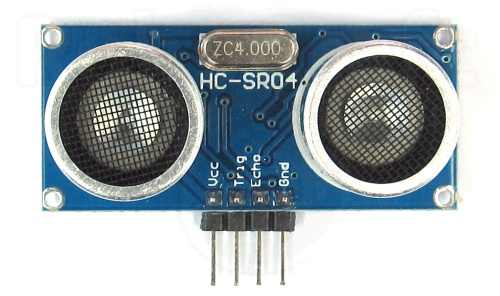
\includegraphics[width=.3\linewidth]{images/hcsr40.jpg}
	\caption{The specific ultrasonic sensors are 3 \textbf{HC-SR04}.\cite{hcsr40datesheet}}
	\label{fig:ultrasonic_pic}
\end{figure}

To avoid damaging the Raspberry pi when using these ultrasonic sensors, a voltage divider was needed in order to protect its input pins. The ultrasonic sensor operates at 5V, resulting in the output from the sensor being 5V. The GPIO ports on the Raspberry Pi operate at 3.3V, so the voltage divider is used to limit the voltage going into the input port from the ultrasonic sensor, while still providing a correct \textit{input-HIGH} signal to the Raspberry Pi.
When the sensors are initially powered on they require a few milliseconds to initialize, before they can be used to take measurements. This is recommended in the datasheet\cite{hcsr40datesheet}.


The HC-SR04 operates using 4 pins: Vcc, Trigger, Echo, Gnd.
The trigger pin on the sensor is connected to the Raspberry Pi as an GPIO-output and the echo pin is connected as a GPIO-input. The echo pin outputs a 5V signal, so to protect the Raspberry Pi we have created the following setup:

\begin{figure}[H]
	\centering
	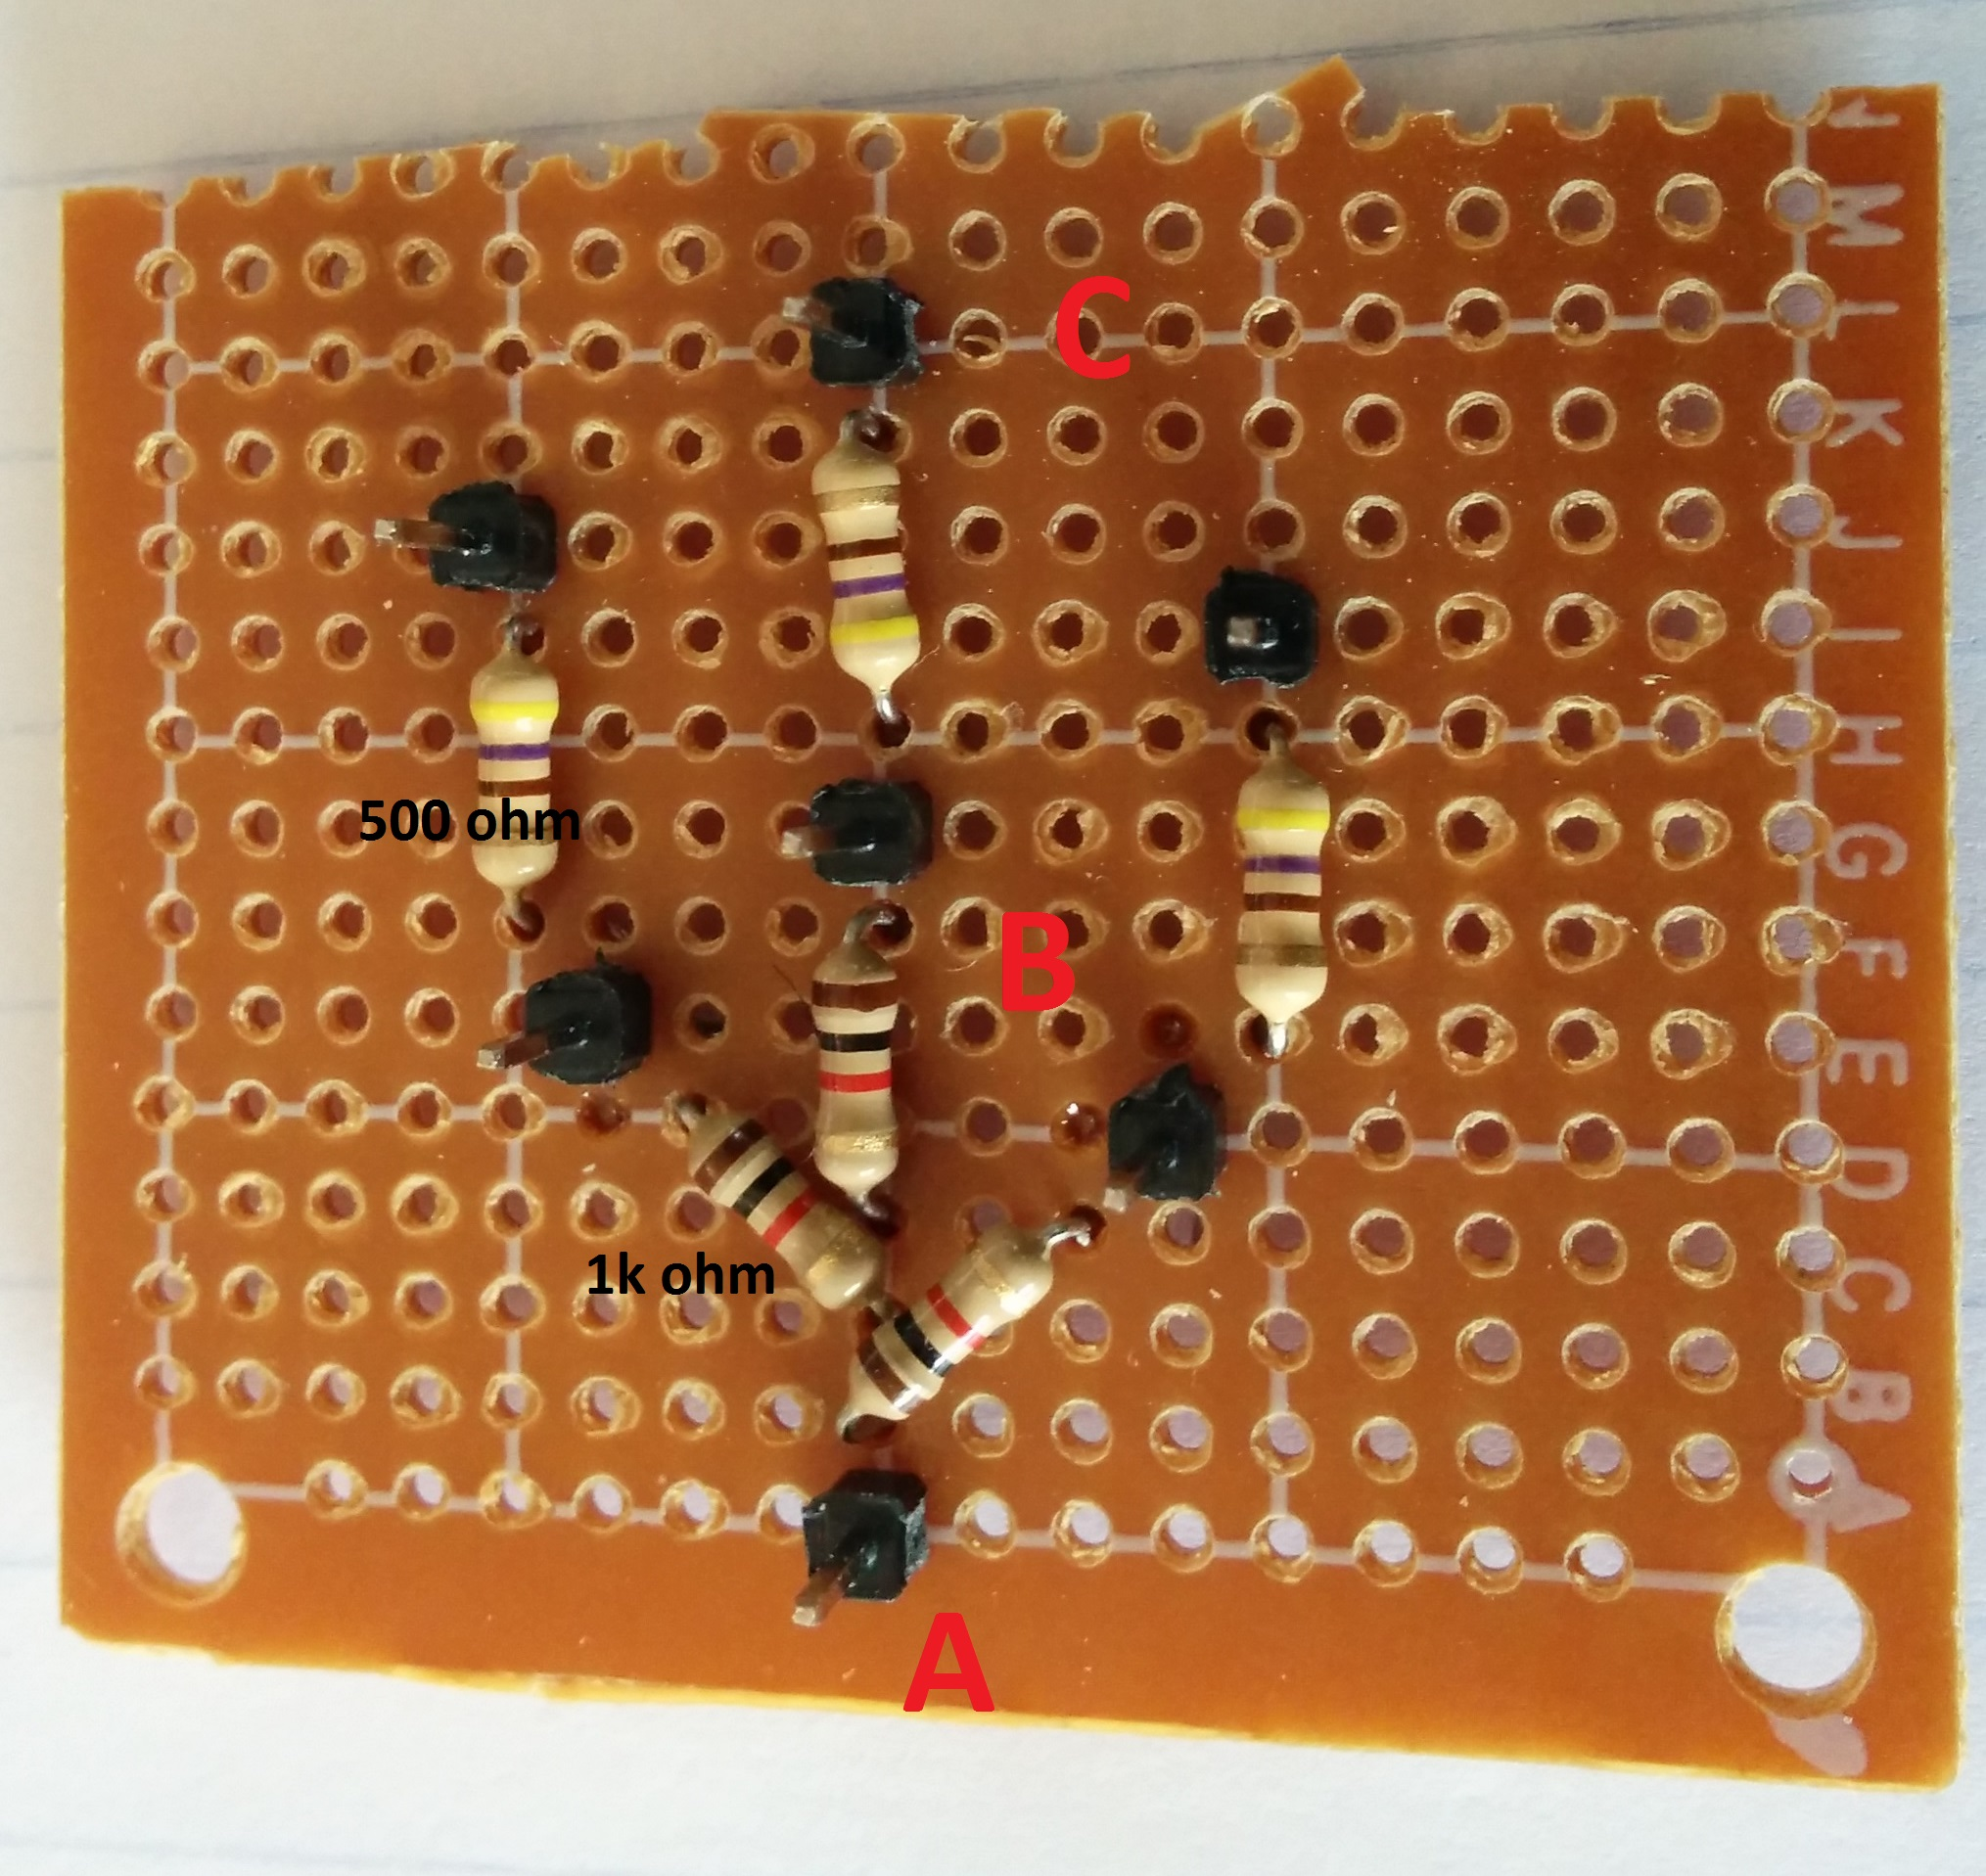
\includegraphics[width=.3\linewidth]{images/vd_labelled.jpg}
	\caption{Picture of the voltage dividers}
	\label{fig:voltagedividers}
\end{figure}

The circuit in figure \ref{fig:voltagedividers} has three sets of voltage dividers. Besides protecting the Raspberry Pi from the 5V, there are also other advantages of the board. Instead of using 12 pins for the three ultrasonic sensors the board reduces it to only end up using 8 pins, since the board above combines their 5V Vcc's and the ground pins into two common pins.  
The three pins at the top of the figure labeled C are the output pins from the ultrasonic sensors, which at that time has a voltage of 5V. The pins labeled as B is where the Raspberry Pi is connected, the voltage divider has at this point reduced the voltage to the suitable 3.3V for the Raspberry Pi. \\ 
The final pin labeled C is the common ground for the three voltage dividers.

\begin{figure}[H]
	\centering
	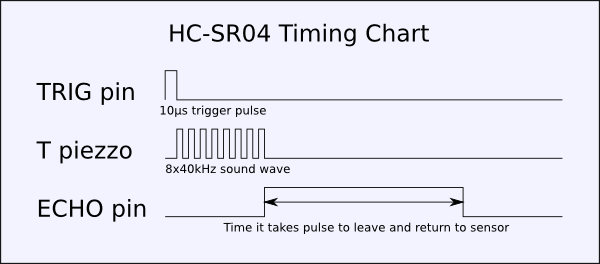
\includegraphics[width=.45\linewidth]{images/hcsr04timingchart.png}
	\caption{The HC-SR04 timing chart\cite{hcsr04timingchart}}
	\label{fig:timingchartpic}
\end{figure}

To retrieve a distance measurement, a 10$\mu$s pulse is sent from the sensor using the trigger pin, the echo pin then receives a HIGH-pulse equivalent to how long it took to hear the echo. This means that length of this high$-$pulse is proportional to how far away the object is that distance is being measured between\cite{ultrasonichowitworks}.

\lstinputlisting[firstline=31, lastline=49, title=ultrasonic.py, language=Python]{../code/autonomous-rover/triple-ultrasonic-test.py}

The snippet of code above is the function that retrieves the distance measurement between the ultrasonic sensor module and the current object in front of it.
On line 3, the trigger output is set to High for 10$\mu$s to create the ultrasonic burst. When the burst returns the input pin ECHO goes high for the duration of the pulse, which is measured by the subtracting the stop time from the start time.
The distance is returned in centimetres, since the speed of sound ($340m/s$) has been converted to centimetres per second.
